\documentclass[12pt, paper=a4]{elsarticle}

\makeatletter
\def\ps@pprintTitle{%
	\let\@oddhead\@empty
	\let\@evenhead\@empty
	\def\@oddfoot{\centerline{\thepage}}%
	\let\@evenfoot\@oddfoot}
\makeatother

\usepackage{amsmath,xcolor,todonotes,graphicx,marvosym,dsfont,import,fullpage,textcomp,colortbl,array,pgfplots,lscape}
\usepackage{caption}
\definecolor{grey}{gray}{0.5}
\definecolor{lightgrey}{gray}{0.8}
\usepackage{amsmath}
\usepackage[colorlinks=true, linkcolor=black, citecolor=black, urlcolor=black]{hyperref} 
%\usepackage[authoryear]{natbib}
\usepackage{siunitx}
\usepackage{float}
%\numberwithin{equation}{section}
%\numberwithin{figure}{section}
%\numberwithin{table}{section}
\graphicspath{ {Figures/} }
\usepackage{tabularx} 
\usepackage{lscape}
\usepackage{pdfpages}
\usepackage[titletoc,toc,title]{appendix}
\usepackage{array}
\newcolumntype{L}[1]{>{\raggedright\let\newline\\\arraybackslash\hspace{0pt}}p{#1}}
\newcolumntype{C}[1]{>{\centering\let\newline\\\arraybackslash\hspace{0pt}}p{#1}}
\newcolumntype{R}[1]{>{\raggedleft\let\newline\\\arraybackslash\hspace{0pt}}p{#1}}
\graphicspath{ {fig/} }
\bibliographystyle{apalike} 
% Adriviations to make life eaiser



\newcommand{\St}{Spatio-temporal\xspace}
\newcommand{\koe}{Koenigsberger model\xspace}


\DeclareRobustCommand{\bigO}{\text{\usefont{OMS}{cmsy}{m}{n}O}}






% Test

\setcounter{topnumber}{2}
\setcounter{bottomnumber}{2}
\setcounter{totalnumber}{4}
\renewcommand{\topfraction}{0.85}
\renewcommand{\bottomfraction}{0.85}
\renewcommand{\textfraction}{0.15}
\renewcommand{\floatpagefraction}{0.8}
\renewcommand{\textfraction}{0.1}
\setlength{\floatsep}{1pt plus 2pt minus 2pt}
\setlength{\textfloatsep}{1pt plus 2pt minus 2pt}
\setlength{\intextsep}{1pt plus 2pt minus 2pt}
\usepackage{acronym}
\usepackage{cleveref}
\newcommand\numberthis{\addtocounter{equation}{1}\tag{\theequation}}
\usepackage{chemformula}
\usepackage{subcaption}
\usepackage{ upgreek }
\definecolor{mygreen}{RGB}{0, 128, 0}

%\linespread{2}

\usepackage{tabularx} 
\usepackage{ amssymb }
\usepackage{mathtools}
\usepackage{color}
\usepackage{xspace}
\usepackage{bm}

\usepackage{titlesec}
\titleformat{\section}
{\normalfont\bfseries}{\thesection}{1em}{}

\titleformat{\subsection}
	{\normalfont\scshape\bfseries}{\thesubsection}{1em}{}
	
\setcounter{secnumdepth}{2}
\titleformat{\subsubsection}
	{\normalfont\scshape\bfseries\itshape}{\thesubsubsection}{1em}{}


\begin{document}
	
%\begin{acronym}[UML] %or [TDMA]
	
	\acrodef{rbc}[$\mathrm{RBC}$]{Red Blood Cell }
	\acrodef{hs}[$\mathrm{HS}$]{Hereditary Spherocytosis }
	\acrodef{o2}[$\mathrm{O_2}$]{Oxygen }
	\acrodef{dmv}[$\mathrm{DMV}$]{Donnell-Mushtari-Vlasov }
%\end{acronym}







	
	\begin{frontmatter}
		\title{{Modification of Surface Stability Equation to Suit Red Blood Cells (RBC) with \acf{hs} } }
		
		\author{\underline{Michelle Goodman}\footnote[1]{University of Canterbury, Tsinghua University Exchange, \href{mailto:michelle.goodman@canterbury.ac.nz}{michelle.goodman@canterbury.ac.nz}}$~$, 
			Steve Xiangthu\footnote[2]{Tsinghua University}$~$, 
			Bing Wang\footnotemark[2]$~$,}
		
			
		\begin{abstract}
			\ac{hs} is a disorder that affects the physical shape of the \ac{rbc} in the human body causing them to become spherical in shape. Patients with \ac{hs} often experience anemia as a side affect from the increased rate of degeneration of \ac{rbc} with symptoms of fatigue, shortness of breath, irritability, dizziness or lightheadedness, increased heart rate, headache and heart palpitations. The deformation of spherical \ac{rbc}s leads to the increased rate of degeneration and is, thus, highly important to understand. This research looks to modify surface stability mathematical relationships to suit the physiological make up of a \ac{rbc}. Three possible approximations were chosen to explore and suitable mathematical relationships defining the surface stability were generated. For each of the options had associated benefits and disadvantages with no option being able to be validated without extensive additional research. 
		\end{abstract}
		
		\begin{keyword}
			RBC \sep Hereditary spherocytosis \sep Surface stability \sep Amplitude of perturbation 
			
		\end{keyword}
	\end{frontmatter}
	
	%\section{Introduction}


\noindent  
Procedure will be
\begin{enumerate}
	\item Start with simple problem and understand the equations
	\item	Research into the composition of a RBC
	\item	Adapt the simple problem to suit the RBC
\end{enumerate}

\noindent Deduce the stability analysis of the equation for the intricate problem 
\begin{itemize}
	\item Look into PHD thesis to understand the formulation of the equation
\end{itemize}

\noindent Need properties of the red blood cell
\begin{itemize}
	\item Including membrane and
	\item Cytoplasm
\end{itemize}





\begin{figure}[H]
	\centering

		
\includegraphics[width=0.5\linewidth]{fig/ele}

	\caption{This is my ele  }
	\label{fig.ele}
\end{figure}


	
	\section{Red Blood Cells Composition} \label{Sect.Blood}


\noindent There are around 25 trillion \ac{rbc} within the human body \cite{Cimen2008}. A \acf{rbc} is scientifically known as an erythrocyte, the word has Greek origins with erythros meaning red and -cyte meaning cell. A \ac{rbc}'s principle purpose is to deliver \ac{o2} to the body tissue via blood flow in the circulatory system. In humans, \ac{rbc} take up oxygen in the lungs and release it into tissues while squeezing through the body's capillaries. The dynamic shape of the \ac{rbc} is critical to the transportation and release of \ac{o2} within the blood stream and is if great importance to understand.

A typical healthy \ac{rbc} comprises of only 2 main parts: the cytoplasm and the cell membrane. The cytoplasm of erythrocytes is rich in hemoglobin. Hemoglobin is an iron-containing biomolecule that binds to oxygen and is responsible for the distinct red colour \cite{Shape2010}. The cell membrane is composed of proteins and lipids that control the inflow and outflow of the cell along with the physical properties essential for deformability and structural stability. Unlike almost all other cells in the human body \ac{rbc}s `anucleate' when mature, this means that they lack a cell nucleus \cite{redblood2009}. In addition, \ac{rbc}s also lack other intracellular organelles. These deficits enhances the ability for a \ac{rbc} to deform when traversing the circulatory system and specifically the capillary network.


A healthy, mature  \ac{rbc} is shaped as an oval biconcave disk. They are often viewed as `sacks of hemoglobin, with a plasma membrane'. Approximately 2.4 million new erythrocytes are produced per second in human adults \cite{Minasyan2014} and have a life of around 100–120 days \cite{Minasyan2014, Kim1979} before being recycled within the body. Each circulation takes about 60 seconds in which an erythrocyte will intake \ac{o2} in the lungs, be pumped by the heart, traverse the circulatory system to the desired location, enter the capillary network in which the \ac{rbc} will deform releasing the \ac{o2}, then, finally, return to the lungs via the heart \cite{Minasyan2014, Kim1979}. 

A typical human \ac{rbc} has a disk diameter of approximately $6.2–8.2 \mu m$ \cite{Shape2010} and a thickness at the thickest point of 2–2.5$\mu m$ with a minimum thickness in the centre of 0.8–1$\mu m$ \cite{Shape2010}. These cells have an average volume of about $90 f$L ($1f$L$ = 10^{-15}$L) with a surface of about 136 $\mu m^2$ \cite{Shape2010}. A \ac{rbc} can swell up to a sphere shape containing $150 f$L, without membrane distension \cite{Minasyan2014}.


\subsection{Membrane composition}
\noindent \ac{rbc} membrane plays a key role in the cells ability to deform, flex, adhere to other cells and to interface with immune cells. The abilities of each are dependent on the specific membrane composition. A \ac{rbc} membrane is composed of 3 layers. The glycocalyx on the exterior, which is rich in carbohydrates, the lipid bilayer which contains many transmembrane proteins alongside its lipidic main constituents and the membrane skeleton, a structural network of proteins located on the inner surface of the lipid bilayer \cite{redblood2009, Shape2010} (Figure \ref{fig.rbc.wall}). 

\begin{figure}[H]
	\centering
	
	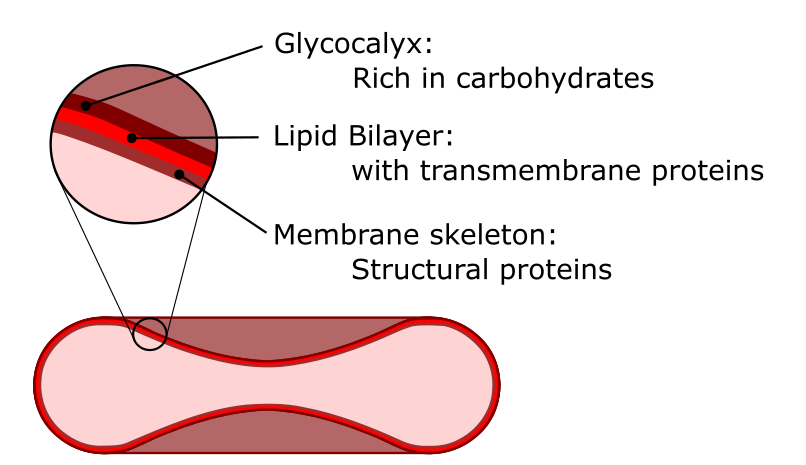
\includegraphics[width=0.5\linewidth]{fig/rbc}
	
	\caption{Pictorial of a cross-section of a \ac{rbc} with zoom on the membrane comprising of three layers. Image created by M. Goodman  }
	\label{fig.rbc.wall}
\end{figure}

\noindent The outer monolayer is comprised of Phosphatidylcholine (PC) and Sphingomyelin (SM) compared to the inner monolayer which is comprised of Phosphatidylethanolamine (PE) small amounts of Phosphoinositol (PI) and Phosphatidylserine (PS) \cite{Quinn2002}. Note, in this research only, all the layers of the cell membrane will be referred to as the cell wall.


\subsubsection*{Membrane lipids}
\noindent The membrane is similar to other cells in the human body and is not unique to the \ac{rbc}. The \ac{rbc} membrane comprises a typical lipid bilayer, composed of cholesterol and phospholipids in equal proportions by weight \cite{redblood2009} (Figure \ref{fig.rbc.lipid}). The composition of the lipid bilayer defines many physical properties including the membrane permeability and fluidity. The lipids in the bilayer also help regulate the activity of many membrane proteins.

\begin{figure}[H]
	\centering
	
	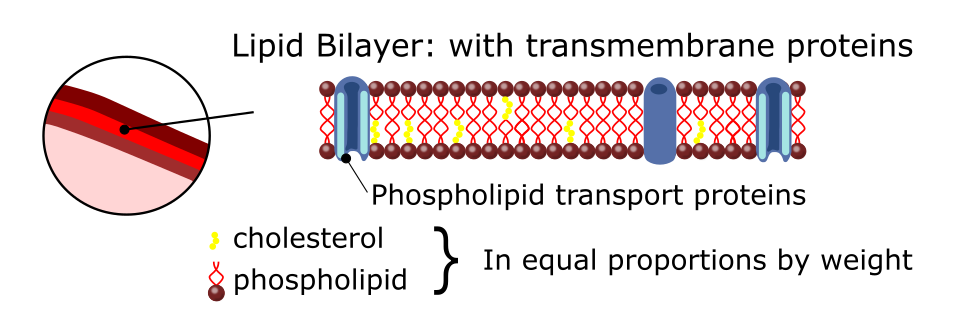
\includegraphics[width=0.8\linewidth]{fig/Lipidbylayer}
	
	\caption{Pictorial of \ac{rbc} cell membrane, lipid bilayer detail including cholesterol, phospholipids and transport proteins. Image created by M. Goodman }
	\label{fig.rbc.lipid}
\end{figure}


\subsubsection*{Membrane proteins}
\noindent The proteins of the membrane skeleton, responsible for the deformability, flexibility and durability, enable a \ac{rbc} to squeeze through capillaries less than half the diameter of the \ac{rbc} and recovering the discoid shape as soon as these cells stop receiving compressive forces. There are currently more than 50 different types of membrane proteins, with a possible of a few hundred to a million copies per \ac{rbc} \cite{redblood2009}. Approximately 25 of these membrane proteins carry the various blood group antigens, such as the A, B, Rh antigens, etc \cite{redblood2009}. The membrane proteins perform a wide diversity of functions such as transporting ions and molecules across the red cell membrane, adhesion, interaction with other cells (endothelial cells), signaling receptor and many others \cite{redblood2009}. Problems with the proteins in these membranes are associated with multiple disorders, such as hereditary spherocytosis, hereditary elliptocytosis, hereditary stomatocytosis, and paroxysmal nocturnal hemoglobinuria.

\subsection{Hereditary Spherocytosis (HS)} \label{Sect.HS}
\noindent \ac{hs}  is a congenital \ac{rbc} membrane disorder characterized by spherical \ac{rbc}s that have reduced diameter (microspherocytosis) and are intensely hemoglobinized (carrying more hemoglobin than normal) \cite{Shape2010}. \ac{hs} is the most common hereditary \ac{rbc} membrane disorder found and affects approximately 1 in 2,000 individuals of northern European ancestry \cite{redblood2009}. \ac{hs} is caused by heterogeneous defects in proteins that vertically connect the membrane skeleton to the lipid bilayer\cite{redblood2009} (see Figure \ref{fig.rbc.wall}). Interactions dependent on vertical connection are thought to play a role in the mechanical stability of the \ac{rbc} membrane \cite{Shape2010}. \ac{hs} causes a loss of spectrin density resulting in a greater maximum stretch that a membrane can undergo beyond which it is unable to recover to its original shape. Spectrin network connectivity can be as low as 3.3 spectrin per actin for cases of \ac{hs} compared to ~5 spectrin molecules bound to each actin filament \cite{redblood2009,Shape2010,Minasyan2014}. The process of \ac{rbc} surface area loss happens more rapidly than volume loss, which results in the formation of spherical \ac{rbc}s with decreased deformability. In healthy patients \ac{rbc}s with decreased membrane surface area are unable to effectively traverse the spleen and are subsequently removed from circulation by the spleen \cite{Shape2010}. The changes seen in \ac{hs} \ac{rbc}s are also seen in non-hereditary spherocytosis, however, typically less severe.

For the purposes of this research, the \ac{rbc} modelling approximations will be modelled after a spherical \ac{rbc} with any properties not obtainable from a \ac{hs} \ac{rbc} will be approximated as a healthy \ac{rbc}.


\subsection{Cell Properties}
\noindent There are many measurable and derived properties of a cell from experiments and accepted modelling techniques. Here a short overview of related properties is given. Table \ref{table.rbc.prop} contains the physical properties of a healthy blood cell. These properties were found by \citet{ademiloye2016} using approximation methods and computer simulations to give the best results. Thus, these properties are dependent upon on two parameters; $k_a$ and $k_v$ the area and volume constraint respectively. These values were also compared to literature and found to reasonable approximations. 
\\
\noindent
\begin{table} [H]
	\begin{center}
		\caption{ Physical properties of a healthy \ac{rbc} membrane where the area and volume constraints, $k_a$ and $k_v$ respectively are equal.   \ }
		\label{table.rbc.prop}
		\begin{tabularx} {0.95\textwidth}{L{7cm} R{1.5cm} R{1.5cm} R{1.5cm} R{1.5cm} }
			\hline
			\multicolumn{1}{l}{\textbf{Elastic Properties}} & \multicolumn{4}{c}{\textbf{$k_a = k_v = \xi$}}  \\ 
			\multicolumn{1}{l}{\textbf{(Symbol [units])}} & \textbf{$0$} & \textbf{$ 100$} 	& \textbf{$ 150$} 	& \textbf{$300$}  \\  
			\hline
			\multicolumn{1}{l}{Young's Modulus (E) $[\mu Nm^{-1}]$}			  & 22.13 				& 21.42 			& 19.31 		 	& 17.31 \\
			\multicolumn{1}{l}{Poisson's Ratio ($v$) }						  &	0.33 				& 0.46 				& 0.45 			& 0.44 \\
			\multicolumn{1}{l}{Shear Modulus ($\mu _h$) $[\mu Nm^{-1}]$}	 &		7.98 			&		7.49 		& 6.70 	&				6.00 \\
			\multicolumn{1}{l}{Area Compression Modulus ($K) [\mu Nm^{-1}]$} &	15.96 				&		20.14 		& 17.65 &				15.55 \\
			\multicolumn{1}{l}{Bending Modulus (B) $[\times 10^{-14}$ J]}	 &	 6.26				&		 5.87 		& 5.25 	&				4.71 \\
			\hline
			
		\end{tabularx}
	\end{center}
\end{table}

\noindent Arterial blood pressure is found at the maximum state (systole) to be 13-18 kPa and in the minimum state (diastole) to be 8-12 kPa. Note the common unit for arterial blood pressure is millimetres of mercury. 

Finally, average dimensions of a \ac{rbc} need to be considered. A healthy \ac{rbc}s has a diameter of 6.2 to 7.2 $\mu m$ \cite{redblood2009,ademiloye2016,Shape2010,Kim1979,HHSPublic2016} with a \acf{hs} \ac{rbc} being less than this. The cell wall thickness is of the order 100 A \cite{Fung1968} (where 1 Angstrom (A) is a unit of length equal to $10^{-10} m$)  i.e. $100 \times 10^{-10} m = 10^{-8} m = 10 nm$ or the ratio of cytosol radius to wall is approximately 360:1. 



	\section{Stability Equation Source Material} \label{Sect.SE}
\noindent The primary objective of this research is to formulate a surface stability equation for a \ac{rbc} similar to that described by \citet{Prosperetti1974} and further used by \citet{Zeng2018}. In order to understand this further the work by \citet{Zeng2018}, a detailed review of the equation and simplification is supplied here. 

The amplitude of perturbation equation, often refereed to as a surface stability equation (Equation \ref{eq.der.big}) attempts to describe reaction in motion for the interface between a liquid and a gas. Equation \ref{eq.der.big} is derived from the Navier-Stokes equations and incompressibility conditions. \citet{Zeng2018} in particular looks at the application of a water droplet of radius $R$, in air, with a bubble of air (radius $R_b$) contained within it. 

\begin{equation} \label{eq.der.big}
\begin{split}
&\left[ \frac{\rho_1}{n} + \frac{\rho_2}{n+1} \right] \ddot{a} + \left[3 \left( \frac{\rho_1}{n} + \frac{\rho_2}{n+1} \right) \frac{\dot{R}}{R} - 2(n-1)(n+2) \frac{\upmu_2 - \upmu_1}{R^2} \right]\dot{a}  \\ & +\left[ \left(  \frac{n+2}{n}\rho_1 - \frac{n-1}{n+1}\rho_2 \right)\frac{\ddot{R}}{R} + (n-1)(n+2)\frac{\gamma}{R^3} + 2(n-1)(n+2)(\upmu_2 -\upmu_1)\frac{\dot{R}}{R^3}  \right] a  \\& + (n-1)(n+1)\frac{\upmu_1}{R} T_1(R,t) - n(n+2)\frac{\upmu_2}{R} T_2(R,t)  \\ & - (n+1)\rho_1\dot{R}R^{-n-3} \int_0^R (s^3-R^3)s^{n-1}T_1(s,t)ds \\ & + n\rho_2 \dot{R}R^{n-2} \int_{R}^{\infty} (s^3 - R^3)s^{-n-2} T_2(s,t) ds = 0 
\end{split}
\end{equation}

\noindent where the subscript `1' and `2' refer to water and air respectively. $\rho$ is the density, $n$ is the order of the spherical harmonic, $\upmu$ is the viscosity and $\gamma$ is the coefficient of surface tension.
\subsection{Simplification}

\noindent Equation \ref{eq.der.big} is very intricate, according to \citet{Zeng2018} two major simplifications can be made to reduce complexity of the water droplet in air. First, in comparison of the densities and viscosities since $\rho_1 >> \rho_2$ and  $\upmu_1 >> \upmu_2$, $\rho_2$ and $\upmu_2$  can be neglected, leaving simply $\rho = \rho_1$,  $\upmu= \upmu_1$. Furthermore, since $T_2(R,t)$ is related to the viscous effects it is also considerably smaller than $T_1(R,t)$ and as such $T_2(R,t)$ can be neglected leaving $T(r,t) = T_1(R,t)$. Equation \ref{eq.der.big} can be rewritten as Equation \ref{eq.der.big2}.

\begin{equation} \label{eq.der.big2}
\begin{split}
& \frac{\rho}{n}  \ddot{a} + \left[3 \frac{\rho}{n} \frac{\dot{R}}{R} + 2(n-1)(n+2) \frac{\upmu}{R^2} \right]\dot{a}  \\ & +\left[ \left(  \frac{n+2}{n}\rho \right)\frac{\ddot{R}}{R} - (n-1)(n+2)\frac{\gamma}{R^3} + 2(n-1)(n+2)( \upmu)\frac{\dot{R}}{R^3}  \right] a  \\& + (n-1)(n+1)\frac{\upmu}{R} T(R,t)   - (n+1)\rho\dot{R}R^{-n-3} \int_0^R (s^3-R^3)s^{n-1}T(s,t)ds  = 0 
\end{split}
\end{equation}
\noindent Second, \citet{Zeng2018} describe how by consideration of initial and boundary conditions $T(R,t)$ and the integral containing $T(R,t)$ can be defined by Equation \ref{eq.der.T} and Equation \ref{eq.der.intT} respectively.

\begin{equation}\label{eq.der.T}
	T(R,t) \approx \frac{2}{n}\left[(n+1)\dot{a} - (n+2)\frac{\dot{R}}{R} a\right]
\end{equation} 

\begin{equation}\label{eq.der.intT}
	\int_0^R \left(1 - \frac{s^3}{R^3}\right)\left(\frac{s}{R}\right)^{n-2} T(s,t)ds \approx \delta \left( 1 - \frac{s^3}{R^3}  \right) \left(\frac{s}{R}\right)^{n-2} T(s,t)\big\rvert_{s=R} = 0
\end{equation}
\noindent Thus, by using Equation \ref{eq.der.T} and \ref{eq.der.intT}, Equation \ref{eq.der.big2} can be rewritten as Equation \ref{eq.der.big3}.

\begin{equation} \label{eq.der.big3}
\begin{split}
& \frac{\rho}{n}  \ddot{a} + \left[3 \frac{\rho}{n} \frac{\dot{R}}{R} + 2(n-1)(n+2) \frac{\upmu}{R^2} \right]\dot{a}  \\ & +\left[ \left(  \frac{n+2}{n}\rho \right)\frac{\ddot{R}}{R} - (n-1)(n+2)\frac{\gamma}{R^3} + 2(n-1)(n+2)( \upmu)\frac{\dot{R}}{R^3}  \right] a  \\& + (n-1)(n+1)\frac{\upmu}{R} \frac{2}{n}\left[(n+1)\dot{a} - (n+2)\frac{\dot{R}}{R} a\right]   = 0 
\end{split}
\end{equation}

\noindent Finally, the Equation \ref{eq.der.big3} can be rewritten cleanly as a second order derivative equation of $a$ for simplicity and solvability (Equation \ref{eq.der.adotdot} to \ref{eq.der.Bn}).

\begin{equation}\label{eq.der.adotdot}
	\ddot{a} + B_n(t) \dot{a} - A_n(t) a = 0
\end{equation}
\noindent where
\begin{equation}\label{eq.der.An}
A_n(t) = -(n+2) \frac{\ddot{R}}{R} - (n-1)n(n+2) \frac{\gamma}{\rho R^3} -(n-1) (n+2) \frac{2\upmu \dot{R}}{\rho R^3}
\end{equation}
\noindent and
\begin{equation}\label{eq.der.Bn}
	B_n(t) = \frac{3\dot{R}}{R} + \frac{2(n-1)(2n+1)\upmu}{\rho R^2}
\end{equation}

\subsection{Relationship to Internal Bubble} \label{Sect.SE.Bub}
\noindent To solve the perturbation Equation \ref{eq.der.adotdot} the outer water radius $R(t)$ and subsequent derivatives are needed. First, the total volume of the water must not change due to an incompressible fluid assumption, ie Equation \ref{eq.bub.V} should hold true.

\begin{equation}\label{eq.bub.V}
R^3 - R_b^3 = R_0^3 - R^3_{b0} 
\end{equation}
\noindent Thus, the derivative of this must also be true (Equation \ref{eq.bub.dV}).

\begin{equation}\label{eq.bub.dV}
R^2\dot{R} - R_b^2\dot{R_b} = 0
\end{equation}
\noindent where in Equation \ref{eq.bub.V} and \ref{eq.bub.dV} the subscript `0' denoted the initial radii. The bubble dynamics are obtained circularly from the unsteady non-linear Bernoulli equation defined in \cite{Zeng2018} (Equation \ref{eq.bub.Rb}).

\begin{equation} \label{eq.bub.Rb}
\ddot{R_b}\left( R_b - \frac{R_b^2}{R} \right) + \dot{R_b}^2 \left( \frac{2}{3} + \frac{4\upmu}{\dot{R_b} R_b \rho} -2\frac{R_b}{R}  + \frac{R_b^4}{2R^4} \right) + \frac{2\gamma}{\rho}\left( R_b^{-1} +R^{-1} \right) = \frac{P_b - P_{\infty}}{\rho}
\end{equation}
\noindent where $P_{\infty}$ is the pressure well away from the system and $P_b$ is the pressure of the gas inside the bubble which is found assuming an adiabatic bubble surface relationship (Equation \ref{eq.bub.Pb}).
\begin{equation} \label{eq.bub.Pb}
P_b R_b^{3\bm{\upgamma}} = P_{b0}R_{b0}^{3\bm{\upgamma}}
\end{equation}
\noindent Finally, where $\bm{\upgamma}$ is the ratio of specific heats.

	\subsection{RBC Modelling Approximation}
\noindent As mentioned in Section \ref{Sect.HS}, this research will focus on spherical \ac{rbc} as starting point. This initial approximation allows the surface stability completed by \citet{Prosperetti1974} and further used by \citet{Zeng2018} to be loosely compared to a \ac{rbc}. However, this comparison between the water droplet and a \ac{rbc} is fundamentally flawed and needs further consideration. 

Figure \ref{fig.rbc.actual} highlights the differences between the water droplet and a \ac{rbc} and identifies the main difficulty in generating a surface stability equation similar to the water droplet material \cite{Prosperetti1974,Zeng2018} for the \ac{rbc}.
\\
\begin{figure}[H]
	\centering
	
	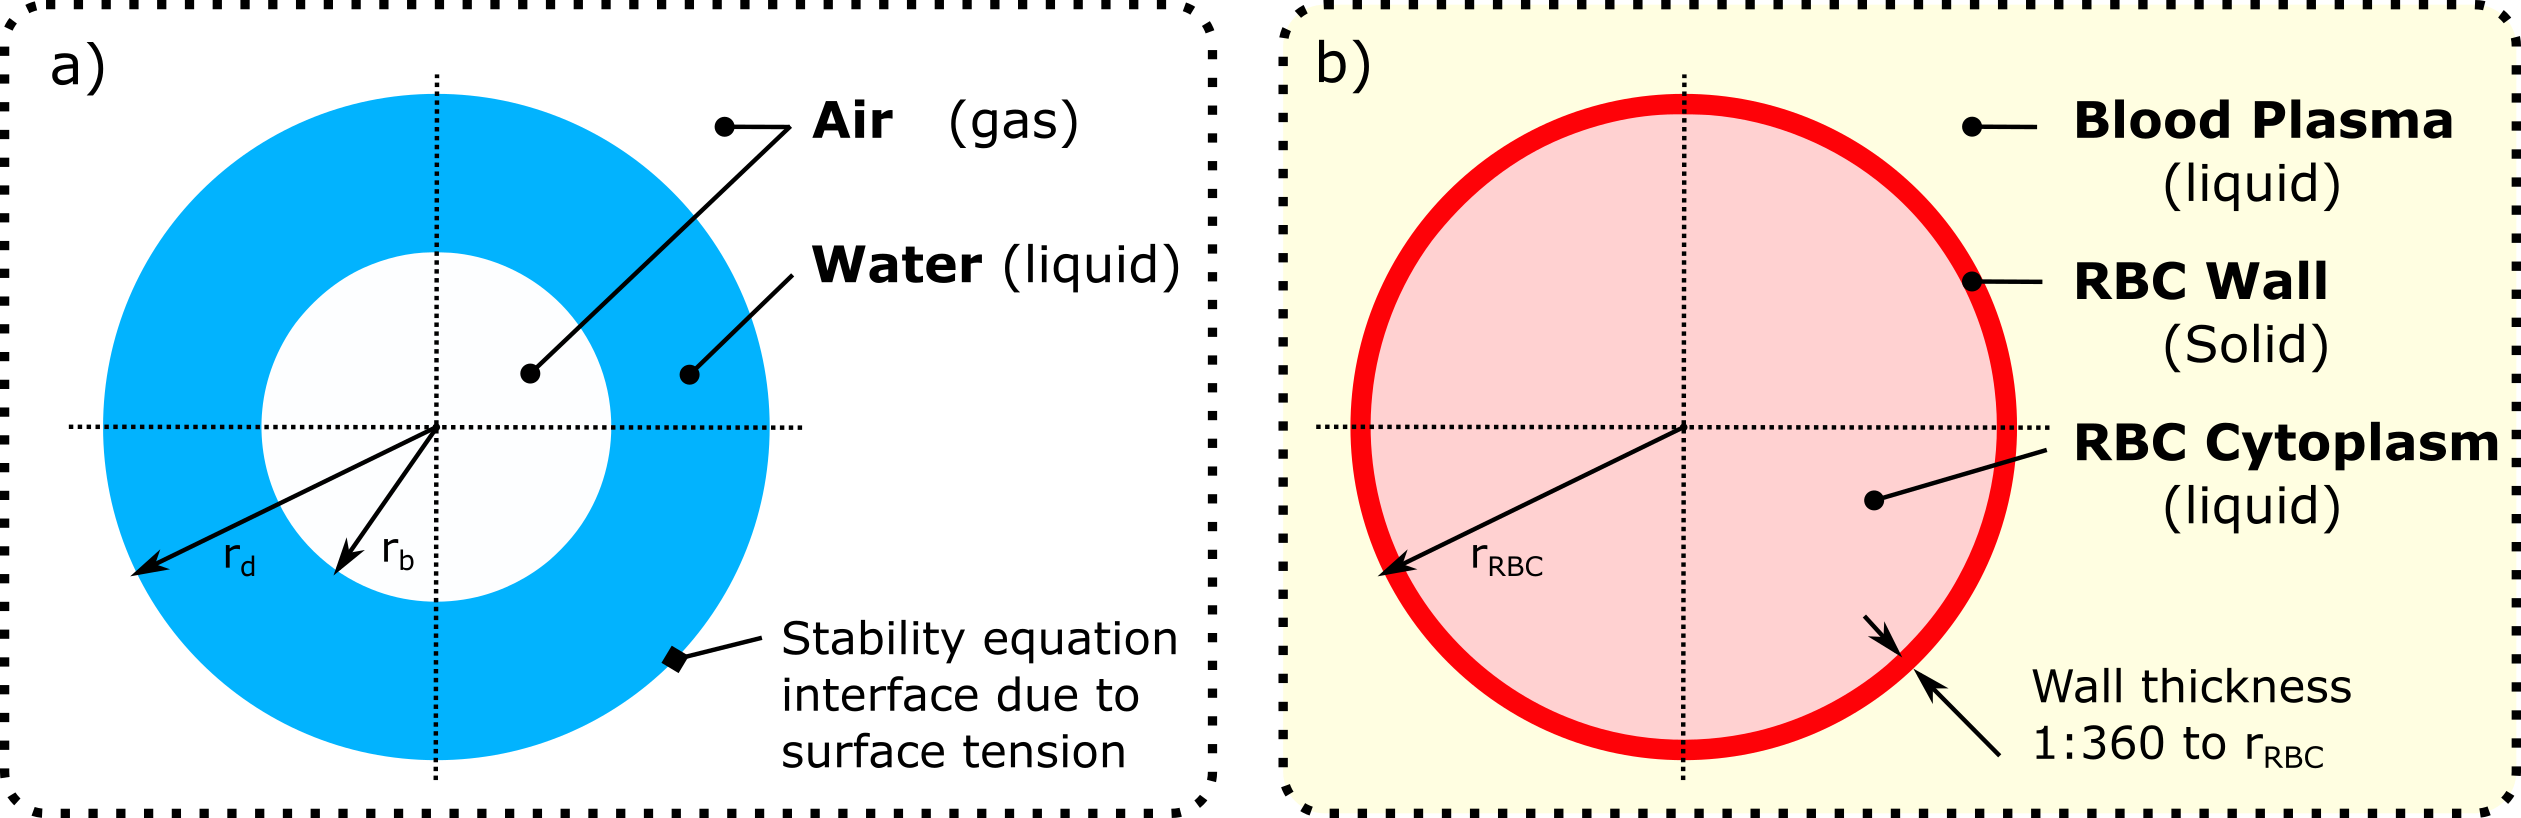
\includegraphics[width=1\linewidth]{fig/Actual}
	
	\caption{Geometry cross-section of a) the water droplet from source material and b) a spherical \ac{rbc}.  }
	\label{fig.rbc.actual}
\end{figure}

\noindent The main difference between the two situations in Figure \ref{fig.rbc.actual} is the occurrence of the solid \ac{rbc} wall. This solid barrier negates the affect of the surface tension between the liquid-gas or liquid-liquid interface. As such changes or simplifications to the \ac{rbc} need to be made to generate a comparable surface stability equation. Figure \ref{fig.rbc.approx} shows three possible approximations of a spherical \ac{rbc} to understand the surface stability. Note, whilst the \ac{rbc} wall is described here as a solid, the cell membrane lipid bilayer is also sometimes referred to a gel-like substance \cite{Himbert2017} who's properties change with temperature. This will be further discussed in Section \ref{Sect.B}. 
\\
\begin{figure}[H]
	\centering
	
	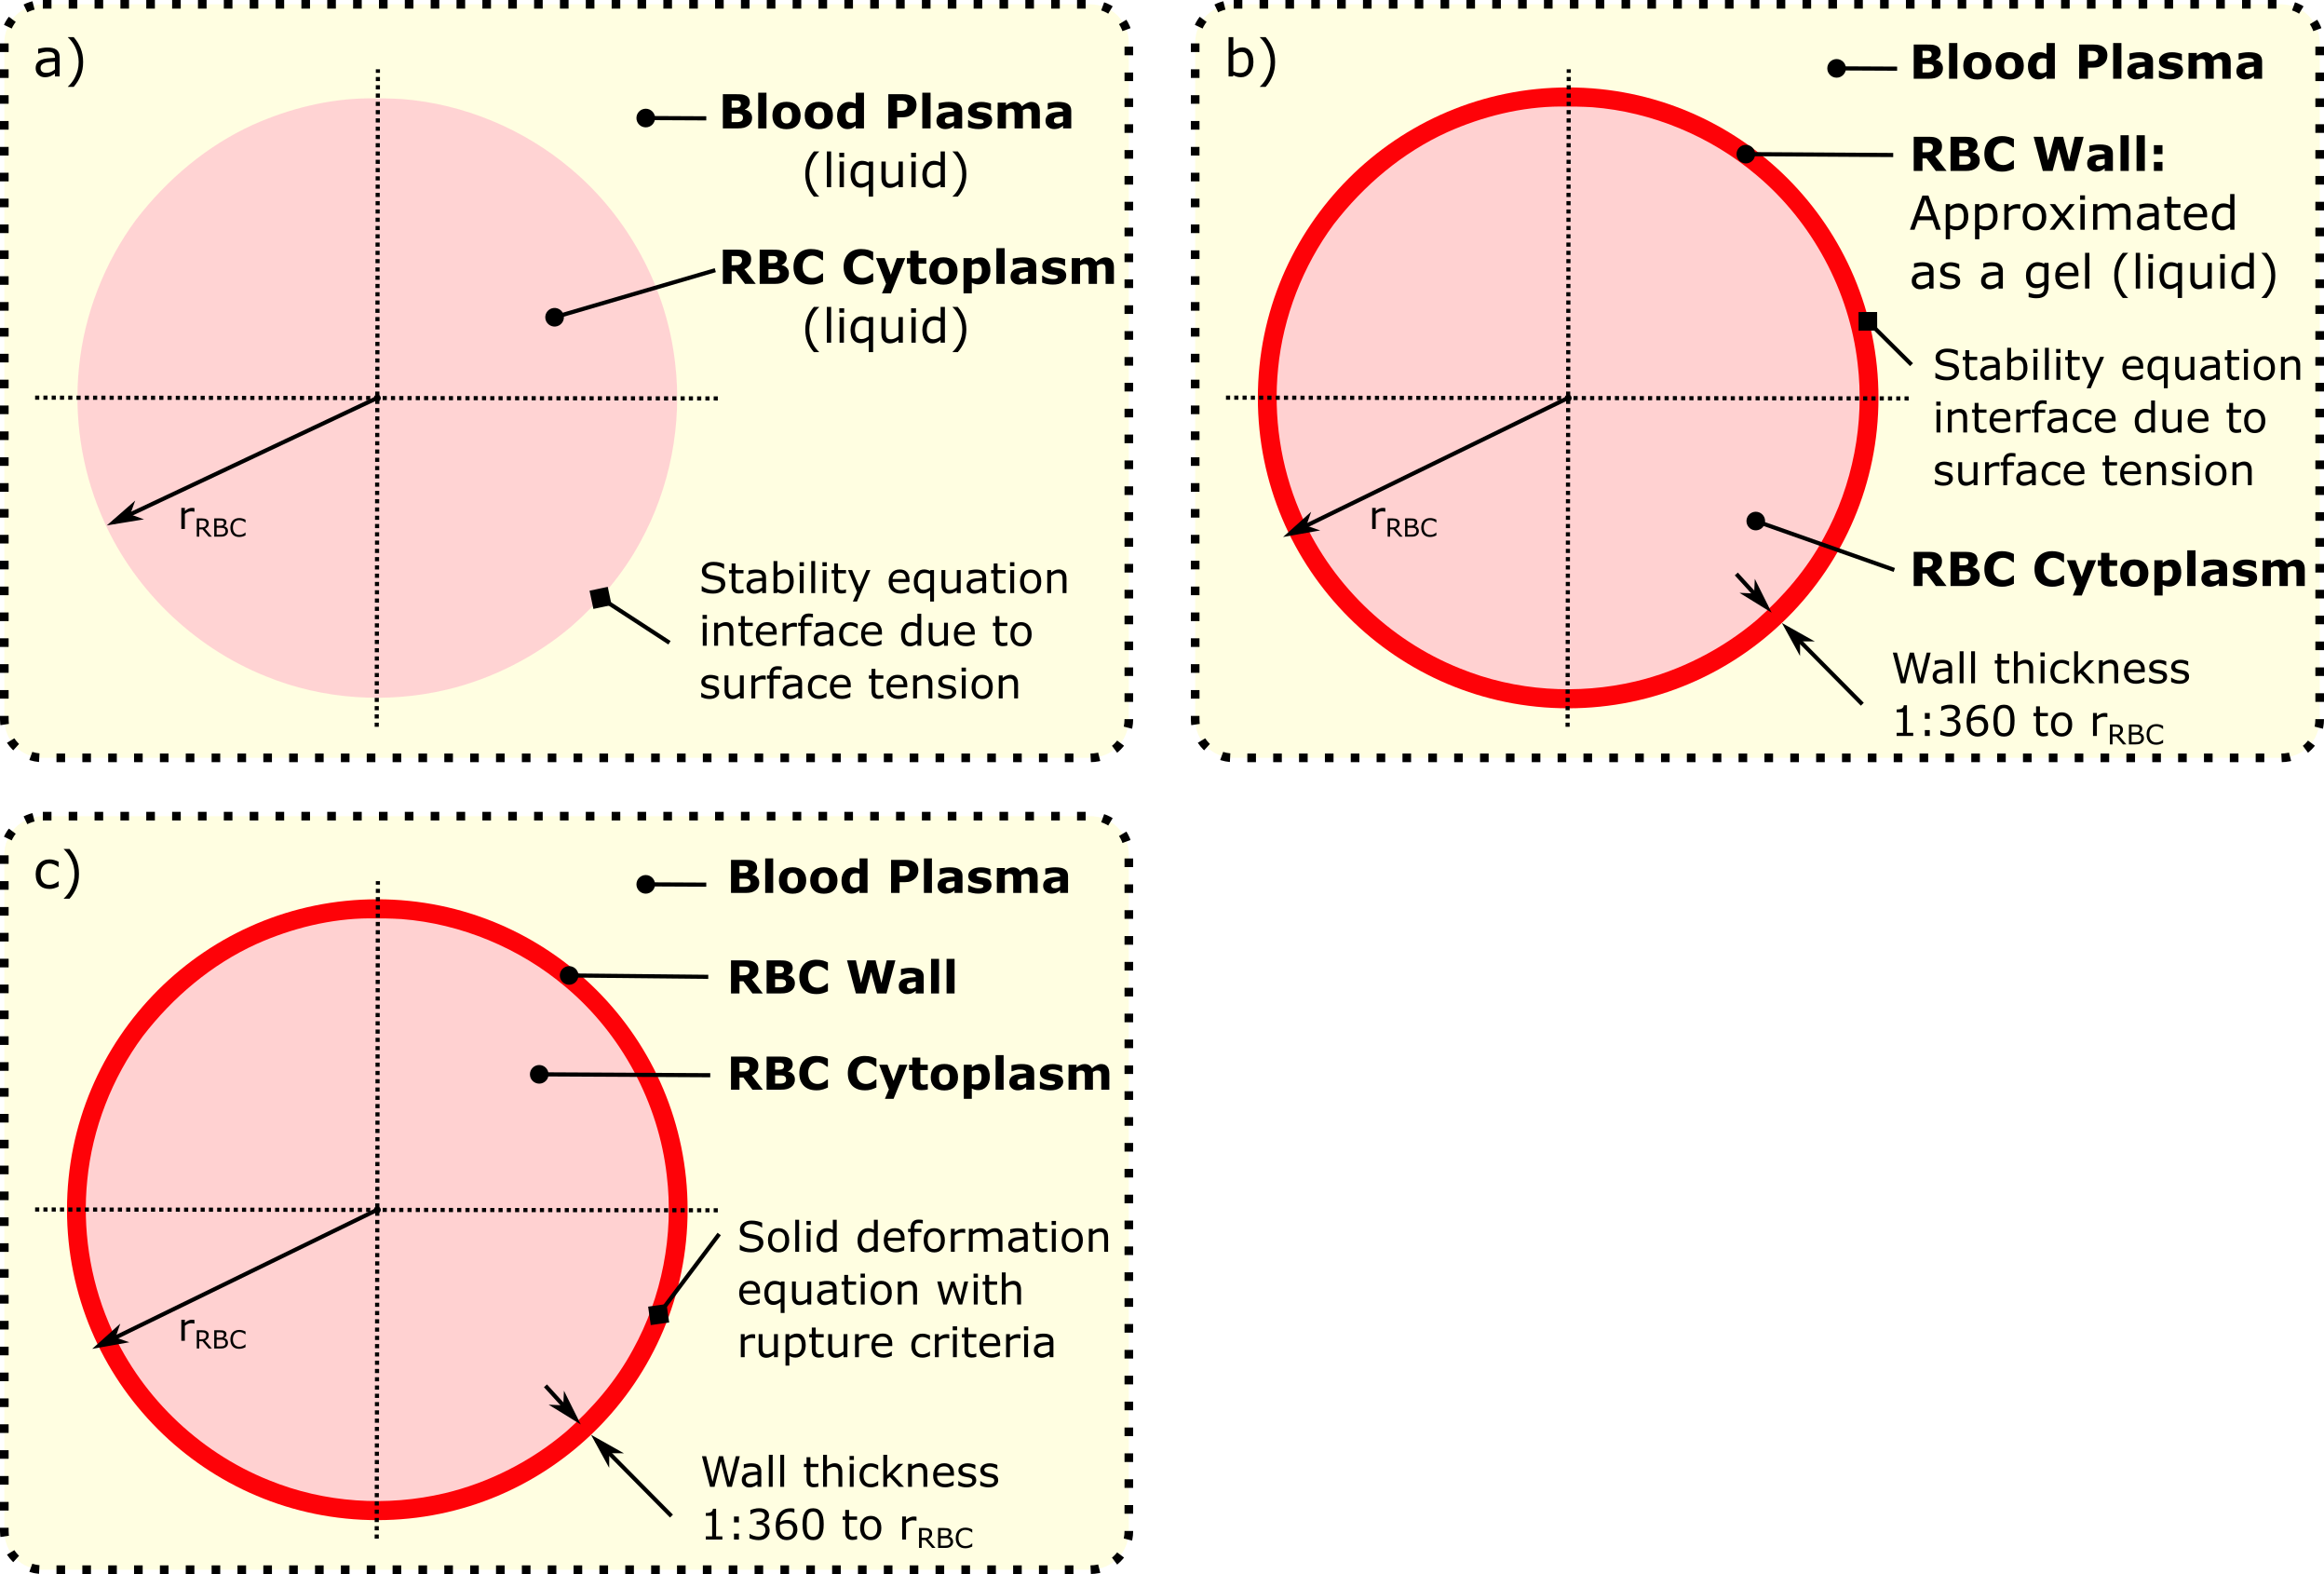
\includegraphics[width=1\linewidth]{fig/approx}
	
	\caption{Possible approximations of the \ac{rbc} in order to generate a surface stability equation. a) makes the assumption that the cell wall is negligible, b) approximates the cell wall as a gel of somewhat comparable properties in order to incorporate the stability equation due to surface tension, and c) substitutes the surface stability equation due to surface tension with a solid deformation equation based upon elastic potential energy.  }
	\label{fig.rbc.approx}
\end{figure}

% How are the two situations differnt
\noindent Each of the three options in Figure \ref{fig.rbc.approx} has associated advantages and disadvantages that need to be considered before implementation. The first of the three options (Figure \ref{fig.rbc.approx}a) assumes that the cell wall can be neglected due to the competitively small thickness when compared to the radius of the cell. This assumption is the least physiological of the three options. However, this assumption allows a direct comparison to the surface stability equation (Equation \ref{eq.der.big}). The second option (Figure \ref{fig.rbc.approx}b) approximates the solid cell wall as a very thin layer of gel liquid instead. The gel approximation allows a similar surface stability equation as \cite{Prosperetti1974,Zeng2018} and option A. For this option it is also assumed that the \ac{rbc} does not rupture as this would result in the model failing. Finally, the third option (Figure \ref{fig.rbc.approx}c) is the most physiological of the three cases, opting to keep the solid cell wall. This option will take a different approach and instead, look at the physical deformation of the cell wall.  However, the disadvantage of the increase in physiological similarity will be increased computation time and mathematical complexity. Again, option C must assume the \ac{rbc} wall does not rupture. 


	\section{Option A} \label{Sect.A}

\noindent From Figure \ref{fig.rbc.approx}a Option A assumes the cell wall is negligible. Given the cell wall thickness, $t_{wall} << r_{RBC}$ it can be assumed that the cell wall plays a negligible role in the surface stability. This is the least physiological of the options as realistically this is not the case. However, there are two main upsides to this assumption. First, rupture criteria does not need to be considered as the dynamics would be the same post rupture and second, the mathematical analysis is directly comparable to the water droplet example in Section \ref{Sect.SE}. 


Here, the surface stability equation (amplitude of perturbation equation) will be re-examined in the context of a \ac{rbc} and associated parameters. Unlike the water droplet in air where by the two mediums have extremely different properties, the blood plasma and the cytoplasm have very comparable properties. Cytoplasm differs from blood plasma primarily by the presence of hemoglobin (Section \ref{Sect.Blood}). Table \ref{table.plasmas} shows the similarities between the cytoplasm and the blood plasma properties.
\\
\begin{table} [H]
	\begin{center}
		\caption{ Summary of main similarities between cytoplasm and the blood plasma properties. \ }
		\label{table.plasmas}
		\begin{tabularx} {0.85\textwidth}{L{4cm} L{1.5cm} | C{3.5cm} C{3.5cm}  }
			\hline
			\textbf{Property (Symbol)} & \textbf{Units} & \textbf{Cytoplasm} & \textbf{Blood Plasma} \\
			\hline
			Viscosity ($\upmu$) & mPa$\cdot$s & $2.27-9.87$ \cite{Tomaiuolo2014} & $1.1–1.3$ \cite{Kesmarky2008} \\
			Density ($\rho$) & kgm$^{-3}$ & $1125 $ \cite{bloodfact2004} & $1025$  \cite{bloodfact2004}  \\
			
			
			\hline			
		\end{tabularx}
	\end{center}
\end{table}

\noindent The two fluids are very similar compared to the differences between water and air and thus, the same simplifications made in Section \ref{Sect.SE} can not be made. Importantly, it is possible that the cytoplasm and the blood plasma will mix due to the comparable densities. This is a major complication and one that needs to be thoroughly considered when choosing this option. For the purpose of this research and to fully explore this option, it is assumed that the two fluids are immiscible (will not mix) on the specified time scale. 


Equation \ref{eq.der.big2} can be simplified to suit a \ac{hs} \ac{rbc} given the similarities in properties in Table \ref{table.plasmas}. First,  $\rho_1 \approx \rho_2$ therefore, $\rho_1 \approx \rho_2 \equiv \rho = 1075$ kgm$^{-3}$. Second, the viscosities will be taken as the average of the ranges, thus, the densities of the cytoplasm and the blood plasma will be $\upmu_1 = 6.07$ mPa$\cdot$s and $\upmu_2 = 1.2$ mPa$\cdot$s respectively. Finally, the small differences between $\upmu_1$ and $\upmu_2$ will lead to even smaller differences between $T_1(R,t)$ and $T_2(R,t)$ and thus, can be approximated as equal, ie $T_1(R,t) \approx T_2(R,t) \equiv T(R,t)$. 


\begin{equation} \label{eq.opta.der1}
\begin{split}
&\left[ \frac{1}{n} + \frac{1}{n+1} \right] \rho \ddot{a} + \left[3 \rho \left( \frac{1}{n} + \frac{1}{n+1} \right) \frac{\dot{R}}{R} - 2(n-1)(n+2) \frac{\upmu_2 - \upmu_1}{R^2} \right]\dot{a}  \\ & +\left[ \rho \left(  \frac{n+2}{n} - \frac{n-1}{n+1} \right)\frac{\ddot{R}}{R} + (n-1)(n+2)\frac{\gamma}{R^3} + 2(n-1)(n+2)(\upmu_2 -\upmu_1)\frac{\dot{R}}{R^3}  \right] a  \\& + T(R,t) \left[ (n-1)(n+1)\frac{\upmu_1}{R} - n(n+2)\frac{\upmu_2}{R} \right]  \\ & - (n+1)\rho_1\dot{R}R^{-n-3} \int_0^R (s^3-R^3)s^{n-1}T(s,t)ds \\ & + n\rho_2 \dot{R}R^{n-2} \int_{R}^{\infty} (s^3 - R^3)s^{-n-2} T(s,t) ds = 0 
\end{split}
\end{equation}

\noindent Next the same boundary conditions are employed such that Equation \ref{eq.der.T} and \ref{eq.der.intT} still hold true. Thus Equation \ref{eq.opta.der1} will now become Equation \ref{eq.opta.der2}.

\begin{equation} \label{eq.opta.der2}
\begin{split}
&\left[ \frac{1}{n} + \frac{1}{n+1} \right] \rho \ddot{a} + \left[3 \rho \left( \frac{1}{n} + \frac{1}{n+1} \right) \frac{\dot{R}}{R} - 2(n-1)(n+2) \frac{\upmu_2 - \upmu_1}{R^2} \right]\dot{a}  \\ & +\left[ \rho \left(  \frac{n+2}{n} - \frac{n-1}{n+1} \right)\frac{\ddot{R}}{R} + (n-1)(n+2)\frac{\gamma}{R^3} + 2(n-1)(n+2)(\upmu_2 -\upmu_1)\frac{\dot{R}}{R^3}  \right] a  \\& + \frac{2}{n}\left[(n+1)\dot{a} - (n+2)\frac{\dot{R}}{R} a\right] \left[ (n-1)(n+1)\frac{\upmu_1}{R} - n(n+2)\frac{\upmu_2}{R} \right]  = 0 
\end{split}
\end{equation}

\noindent which is rearranged to

\begin{equation} \label{eq.opta.der3}
\begin{split}
&\left[ \frac{(2n+1)\rho}{n(n+1)}\right]  \ddot{a} + \left[3 \frac{(2n+1)\rho}{n(n+1)}  \frac{\dot{R}}{R} - 2(n-1)(n+2) \frac{\upmu_2 - \upmu_1}{R^2} \right]\dot{a}   \\& + \frac{2}{nR}(n+1)\left[ (n-1)(n+1)\upmu_1 - n(n+2)\upmu_2 \right]\dot{a} \\ & +\left[ \rho  \frac{4n+2}{n(n+1)} \frac{\ddot{R}}{R} + (n-1)(n+2)\frac{\gamma}{R^3} + 2(n-1)(n+2)(\upmu_2 -\upmu_1)\frac{\dot{R}}{R^3}  \right] a \\& - \frac{2}{n} (n+2)\frac{\dot{R}}{R^2} \left[ (n-1)(n+1)\upmu_1 - n(n+2)\upmu_2 \right]a   = 0 
\end{split}
\end{equation}

\noindent Finally, similar to Equation \ref{eq.der.adotdot}, Equation \ref{eq.opta.der3} can be written as  Equation \ref{eq.opta.adotdot}.

\begin{equation}\label{eq.opta.adotdot}
\ddot{a} + B_n(t) \dot{a} - A_n(t) a = 0 
\end{equation}
\noindent where
\begin{equation}\label{eq.opta.An}
\begin{split}
A_n(t) = & 2 \frac{\ddot{R}}{R} + \frac{n(n+1)}{\rho (2n+1)} \left[ \frac{(n-1)(n+2)}{R^3}\left(\gamma + 2(\upmu_2 -\upmu_1)\dot{R} \right)  - \right. \\ & \left. \frac{2(n+2)\dot{R}}{R^2} \left( \left(n+\frac{1}{n}\right)\upmu_1 - (n+2)\upmu_2 \right) \right]
\end{split}
\end{equation}
\noindent and
\begin{equation}\label{eq.opta.Bn}
\begin{split}
B_n(t) = & 3 \frac{\dot{R}}{R} + \frac{n(n+1)}{\rho (2n+1)} \left[ 2(1-n)(n+2) \frac{\upmu_2 - \upmu_1}{R^2} + \right. \\ & \left. \frac{2(n+1)}{R}\left(\left(n-\frac{1}{n}\right)\upmu_1 - (n+2)\upmu_2 \right) \right]
\end{split}
\end{equation}


\noindent Thus, Equation \ref{eq.der.adotdot} can now be written as Equation \ref{eq.opta.adotdot} to suite a \ac{rbc} with \ac{hs}. ie. the final amplitude of perturbation of the surface is $a = f(t, n, \rho, \mu_1, \mu_2, \gamma, R, \dot{R}, \ddot{R})$.



	\section{Option B} \label{Sect.B}

\noindent Option B approximates the cell wall as a very thin gel-like fluid in order to consider its physiological properties on the structural deformation of a spherical \ac{rbc}.  The gel approximation allows a similar surface stability equation as \cite{Prosperetti1974,Zeng2018} in Section \ref{Sect.SE}. This assumption stems from the Fluid Mosaic Model which describes generic cell membranes as a fluid or gel-like structure at different temperatures \cite{Nicolson2014,Deraitus2001}. However, although the definition describes the membrane as a fluid, fluid like properties such as viscosity (often refereed to as membrane fluidity) are difficult to obtain and thus are often approximated as effective viscosities. 


For this approximation the surface stability equation is described for the membrane to blood plasma interface and the inner interface is found using the same volume conservation, adiabatic surface assumption and unsteady Bernoulli equations found in Section \ref{Sect.SE.Bub}: \textit{Relationship to Internal Bubble}. For this option the subscript `w' will be used to represent the membrane. For the purpose of readability Table \ref{table.plasmas2} describes the blood plasma and cell wall approximated properties.
\\


\begin{table} [H]
	\begin{center}
		\caption{ Summary of main similarities between cytoplasm and the blood plasma properties. \ }
		\label{table.plasmas2}
		\begin{tabularx} {0.8\textwidth}{L{4cm} L{1.5cm} |  C{3cm} C{3cm}  }
			\hline
			\textbf{Property (Symbol)} & \textbf{Units}  & \textbf{Blood Plasma} & \textbf{Wall}\\
			\hline
			Viscosity ($\upmu$) & mPa$\cdot$s  & $1.2$ \cite{Kesmarky2008} & 0.128 \cite{Chang2017,Tran-Son-Tay1984} \\
			Density ($\rho$) & kgm$^{-3}$  & $1025$  \cite{bloodfact2004} & 1040 \cite{Schumacher2009} \\
			
			
			\hline			
		\end{tabularx}
	\end{center}
\end{table}

\noindent Looking at the properties in Table \ref{table.plasmas2}, again, the densities are comparable (only 1.5\% difference) but the viscosities are not. This leads to the same resulting amplitude of perturbation equation as described by Equation \ref{eq.opta.adotdot} with Equations \ref{eq.opta.An} and \ref{eq.opta.Bn}. However, for this scenario, additionally the internal bubble dynamics (Section \ref{Sect.SE.Bub}) are needed.

 For Equation \ref{eq.bub.Pb} the initial pressure of the bubble is assumed to be isotonic ie. $P_{b0} = P_{\infty}$. For Equation \ref{eq.bub.Rb} when the parameters that have no subscript refer to the cell wall. The pressure of the blood plasma can be chosen within the range of typical blood pressures $P_{\infty} \in [8,18]$ kPa and  the effective coefficient of surface tension, is a piecewise function (Equation \ref{eq.opt2.sigma}) depending on the radius from \citet{Dollet2019}.
 
\begin{equation} \label{eq.opt2.sigma}
\gamma = \begin{cases} 
0 & R \leq R_{Buckling} \\
\gamma(R_0) + \frac{d \gamma}{d \ln A}  \left( \frac{R^2}{R_0^2} - 1 \right) & R_{Buckling}\leq R \leq R_{Rupture} \\
\gamma_{Water} & R \geq R_{Rupture} 
\end{cases}
\end{equation}

\noindent where the initial surface tension is approximated as $\gamma(R_0) \in [5,10] \times 10^{-7}$ Jm$^{-2}$ (also equal to N/m) \cite{Safran2005}, $A$ is the \ac{rbc} surface area, $R_{Buckeling}$ is assumed to not occur and $R_{Rupture}$ is a dependent upon the pressure in Section \ref{Sect.CellRupture}.

The potential difficulties with this option is two fold, first, the cell wall rupture (Section \ref{Sect.CellRupture}) and second, the thickness of the cell wall. Until simulations have been complete it is difficult to understand the possible effects the thin cell wall will have on the outcome. To speculate, it is expected that the simulation tolerances need careful consideration in addition to appropriate time step and position mapping needing a higher level of detail for accuracy. 

\subsection{Cell Wall Rupture} \label{Sect.CellRupture}
\noindent Due to the addition of the cell wall dynamics it is important to consider the cell wall rupture. Should the cell wall rupture the dynamics described above become null and void and thus, Option A (Section \ref{Sect.A}) dynamics take over. 

The threshold shear stress, above which extensive cell damage which is directly due to shear stress, is $1500$ dynes/cm$^2$ ($0.015$ N/cm$^2$ = $150$ Pa) \cite{Leverett1972}. Therefore, should the pressure on the cell exceed 150 Pa, the cell wall will exhibit extensive damage and rupture. Since this reading is above standard internal pressure it is deduced that for \ac{rbc} rupture the change in pressure across the cell wall must be greater than 150 Pa, ie $|P_b - P_{\infty}  | \geq 150 $ Pa. Note, it is assumed that initially the pressure gradient is isotonic, meaning the osmotic pressure outside the red blood cells is the same as the pressure inside the cells.


	\section{Option C}

\noindent Finally, the third option (Figure \ref{fig.rbc.approx}c) is arguably the most physiological of the three cases, opting to keep the solid cell wall. Unlike the first two options, here a different approach is necessary to switch from surface tension to elastic mechanical deformation. Again, similar to option B, option C must assume the \ac{rbc} wall does not rupture (Section \ref{Sect.CellRupture}).

There exist multiple different mathematical approaches to this option. \citet{Mansoorbaghaei2011}, for example, look at a 3-dimensional model of a shell under an external impact. This type of approach is both computationally expensive and prone to numerical inconsistencies when applied to the thin wall of the cell. Instead, a thin wall approached was chosen. 

The \ac{dmv} \cite{Hutchinson2016} thin shell theory was chosen as a base for this option. Van der Neut 1932 Dutch PhD thesis was the first to show the rigorous demonstration for the buckling sphere under uniform pressure. His work was based upon the Kirchhoff–Love theory of plates as a two-dimensional mathematical model that is used to determine the stresses and deformations in thin plates subjected to forces and moments. This theory is an extension of Euler-Bernoulli beam theory and was developed in 1888 by Love using assumptions proposed by Kirchhoff. The theory assumes that a mid-surface plane can be used to represent a three-dimensional plate in two-dimensional form.

For this approach four approximations are needed \cite{Chang1994}. First, the uniform thickness of the elastic shell, $\ell$, must be significantly smaller than its radius, ie $\ell/R << 1$. Second, the deformations must be small compared to the radius. Third, the radial stress $\sigma_R$ must be negligible and finally, the fibres in the radial direction need to remain non-permanently-deformed during the motion. Note, \citet{Chang1994} and \citet{Anand2016} (and to a lesser extent \cite{Kraus} and  \cite{Turcotte1981}) used the Kirchhoff-Love thin shell theory with although derived from the same original source contains slight modifications in the approximations, assumptions and boundary conditions used. 

The \ac{dmv} theory (succinctly described by \cite{Hutchinson2016} and including the time dependent component of \cite{Vassilev1997}) describes first the equi-biaxial (equal on both axis's) stress ($\sigma$) as a function of the uniform pressure difference ($P$), radius ($R$) and shell wall thickness
($\ell$) is described by Equation \ref{eq.opt3.sigma}.
\begin{equation} \label{eq.opt3.sigma}
\sigma = \frac{1}{2} P \frac{R}{\ell}
\end{equation}
\noindent Deviation from this uniform state in the form $R(t) = R_0 + a(t)Y_{n}$, or otherwise, $a$ is known as the axial displacement amplitude of perturbation and $Y_{n}$ is the spherical harmonic. The well known Airy stress function $\Delta F$ is used to satisfy the in plane equilibrium along with the additional compatibility condition.  The perturbation process leads to a pair of coupled partial differential equations from \ac{dmv} theory governing the buckling (Equation \ref{eq.opt3.w} and \ref{eq.opt3.F}).
\begin{equation} \label{eq.opt3.w}
D \triangledown^4 a + \frac{1}{R} \triangledown^2 \Delta F + \sigma \ell \triangledown^2 a = 0
\end{equation}
\begin{equation} \label{eq.opt3.F}
\frac{1}{E\ell} \triangledown^4 \Delta F - \frac{1}{R} \triangledown^2 a -\frac{\rho R}{E\ell} \ddot{a} = 0
\end{equation}
\noindent where
\begin{equation} \label{eq.opt3.D}
D = \frac{E\ell^3}{12(1-v^2)}
\end{equation}
\noindent and for spherical coordinates the Laplacian operator $\triangledown^2$ is defined by Equation \ref{eq.opt3.del} with $\triangledown^4 = \triangledown^2(\triangledown^2)$.
\begin{equation} \label{eq.opt3.del}
\triangledown^2f  \equiv \frac{1}{r}\frac{\partial^2}{\partial r^2} (rf) + \frac{1}{r^2 \sin \theta} \frac{\partial}{\partial \theta}\left( \sin \theta \frac{\partial f}{\partial \theta} \right) + \frac{1}{r^2\sin \theta} \frac{\partial^2}{\partial \psi^2}f
\end{equation}
\noindent Eliminating $\Delta F$ from Equations \ref{eq.opt3.w} and \ref{eq.opt3.F} gives Equation \ref{eq.opt3.a}
\begin{equation} \label{eq.opt3.a}
\rho \ddot{a} + \triangledown^2  \left( D \triangledown^4 a  + \sigma \ell \triangledown^2 a + \frac{E\ell}{R^2}a   \right) = 0
\end{equation}
\noindent Thus, in order to consider deformation mechanics,  Equation \ref{eq.opt3.a} is recommended to replace Equation \ref{eq.der.adotdot} from Section \ref{Sect.SE}. For comparison to Section \ref{Sect.A} the final amplitude of perturbation of the surface is $a = f(t, n, \rho, E, \ell, v, P, R)$.



	%\section{Validation}


	\section{Concluding Remarks and Future Work}
Here \ac{rbc}'s with \acf{hs} (sphering of the \ac{rbc} causing a reduced diameter) was investigated as a premise to apply surface stability (or amplitude of perturbation) equations to. The primary objective of this research was to formulate a surface stability equation for a \ac{rbc} similar to that described by \citet{Prosperetti1974} and further used by \citet{Zeng2018}. However, it became quickly apparent that the surface stability equation, based upon surface tension, was not directly comparable to a \ac{rbc} and thus, approximations were needed.

This research presented three different approaches to approximate the physiology of a \ac{rbc}; A) negligible cell wall, B) gel cell wall and C) thin shell cell wall mechanical deformation. Options A and B were considered less physiological than C, but, they were able to apply a similar surface stability equation as the source material. Option B and C, although more physiological than option A, were required to also consider cell rupture. Option C was the most physiological of the options, however, this required an alternative approach looking at a the \acf{dmv} thin shell wall approximation to the deformation. The resulting equation included a spatial consideration not previously included and, thus, would significantly increase computation time.   

The three options provide a good range of physiology and computations scale. Unfortunately however, without raw data of a \ac{rbc} under deformation there is no way of validating the provided equations. Additionally, the amplitude of perturbation equations provided here would need to be incorporated within the entire sphere dynamics described in \citet{Zeng2018} to fully understand their impact. This extensive additional research is expected to have multiple difficulties, some of which were described in this research.   

Overall, the results included within this research are a step towards the combination of these two research areas. It is difficult to say which option presented here would be the most suitable going forward as the benefits of physiological accuracy need to be weighted against the disadvantages of computation time and approximations. It is hoped that one day \acf{hs} \ac{rbc}'s can be accurately modelled in order to advance medications to alleviate some of the symptoms associated with \ac{hs}.

	
	%\appendix% I am not sure where I should invoke \appendix
	%\begin{appendices}
	%	\section{The First App} \label{appendix.first}
	%\end{appendices}
	
	
	\bibliography{library} 
\end{document}

